\documentclass[twoside,draft,a4paper]{article}
%\documentclass[twoside,draft,a4paper]{scrartcl}

%\usepackage{showkeys}
\usepackage[british]{babel}
\selectlanguage{british}
\usepackage{a4}
\usepackage{fancyhdr}
\usepackage[final]{graphicx}
\usepackage{wrapfig}
\usepackage{amsfonts}
\usepackage{amsmath}
\usepackage{amssymb}

%%%%%%%%%%%%%%%%%%%%%%%%%%%%%%%%%%%%%%%%%%%%%%%%%%%%%%%%%%%%%%%%%%%%%%%%%%%%%%

\newcommand{\ToDoList}[1]{{
	\vspace{0.5ex}\hrule\vspace{0.5ex}\itshape
	\begin{itemize}#1\end{itemize}
	\vspace{0.5ex}\hrule\vspace{0.5ex}}}
\newcommand{\ToDo}[1]{\ToDoList{\item #1}}
\newcommand{\ortm}{\rule{0.4ex}{1.5ex}\rule[0.55ex]{0.6ex}{0.4ex}}
\newcommand{\crtm}{\rule[0.55ex]{0.6ex}{0.4ex}\rule{0.4ex}{1.5ex}}
\newcommand{\remove}[1]{{\ortm\ #1 \crtm}}

\newcommand{\ur}[1]{{\rm #1}}     % Up-Right, for brackets etc. in italic text

\newcommand{\Arnold}{Arnol$'$d}
\newcommand{\Poincare}{Po\-in\-ca\-r\'{e}}

\newcommand{\R}{{\mathbb R}}
\newcommand{\T}{{\mathbb T}}
\newcommand{\N}{{\mathbb N}}
\newcommand{\Z}{{\mathbb Z}}

%\newcommand{\disc}[1]{\mathfrak{#1}}
\newcommand{\disc}[1]{\mathbf{#1}}

\newcommand{\eps}{\varepsilon}
\newcommand{\om}{\omega}

\newcommand{\scalar}[2]{{\left\langle\:{#1}\:,\:{#2}\:\right\rangle}}
\newcommand{\textscalar}[2]{{\langle\:{#1}\:,\:{#2}\:\rangle}}
\newcommand{\pderiv}[2]{\frac{\partial {#1}}{\partial {#2}}}
\newcommand{\setdef}[2]{\{\:{#1}\:|\:{#2}\:\}}
\newcommand{\from}{\leftarrow}

\newcommand{\class}[1]{\texttt{#1}}

\newtheorem{theo}{Theorem}%[section]
\newtheorem{lemma}[theo]{Lemma}
\newtheorem{defi}[theo]{Definition}
\newtheorem{coro}[theo]{Corollary}
\newtheorem{hypo}[theo]{Hypothesis}
\newcommand{\qed}{{\hspace*{\fill}$\Box$}}
\newenvironment{proof}{\paragraph*{Proof.}}{\qed}
\newenvironment{subproof}{\subparagraph*}{}
%\renewcommand{\theequation}{\arabic{section}.\arabic{equation}}

\newcommand{\fig}{Fig.}
\newcommand{\Fig}{Fig.}
\newcommand{\figs}{Figs.}
\newcommand{\Figs}{Figs.}
\newcommand{\figref}[1]{{\fig~\ref{#1}}}
\newcommand{\Figref}[1]{{\Fig~\ref{#1}}}
\newcommand{\figsref}[1]{{\figs~\ref{#1}}}
\newcommand{\Figsref}[1]{{\Figs~\ref{#1}}}

\newcommand{\tab}{Table}
\newcommand{\Tab}{Table}
\newcommand{\tabs}{Table}
\newcommand{\Tabs}{Table}
\newcommand{\tabref}[1]{{\tab~\ref{#1}}}
\newcommand{\Tabref}[1]{{\Tab~\ref{#1}}}
\newcommand{\tabsref}[1]{{\tabs~\ref{#1}}}
\newcommand{\Tabsref}[1]{{\Tabs~\ref{#1}}}

%%%%%%%%%%%%%%%%%%%%%%%%%%%%%%%%%%%%%%%%%%%%%%%%%%%%%%%%%%%%%%%%%%%%%%%%%%%%%%

\title{\sf Coco - A modularised continuation core toolbox for Matlab}

\author{Harry Dankowicz
\and Frank Schilder\thanks{Supported by EPSRC grant EP/D063906/1.}
}

\date{\today}

\pagestyle{myheadings}
\markboth{F. SCHILDER AND OTHER AUTHOR(S)}
{RUNNING TITLE OF THE MANUSCRIPT}

%%%%%%%%%%%%%%%%%%%%%%%%%%%%%%%%%%%%%%%%%%%%%%%%%%%%%%%%%%%%%%%%%%%%%%%%%%%%%%

%\renewcommand{\baselinestretch}{1.5} % for submission
%\renewcommand{\baselinestretch}{1.2} % for package showkeys

\begin{document}

% titlepage

\thispagestyle{plain}

\maketitle

\begin{abstract}
Text of the abstract.
\end{abstract}

\vspace{1ex}\noindent {\bf Key words.}

\vspace{2ex}\noindent {\bf AMS subject classifications.}

\section*{Copyright}

This preprint was submitted to (name of the Journal).

\tableofcontents

%%%%%%%%%%%%%%%%%%%%%%%%%%%%%%%%%%%%%%%%%%%%%%%%%%%%%%%%%%%%%%%%%%%%%%%%%%%%%%

\section{Introduction}

\section{Review of continuation}

In this section we review the principle of parameter continuation and point out differences to conventional implementations.

\subsection{Setting up the system}

We are interested in families of solutions of the equation $F(x,\lambda)=0$, $F:\R^l \times \R^m \to \R^n$, where $l+m>n$, and want to trace a set of test functions $G(x,\lambda)$ along such families. Note that the above notation includes the traditionally considered cases $l=n$ and $m=0$. Even though these cases are equivalent we did not restrict our toolbox to one of those as to allow the user to choose her favourite problem formulation.

We construct a map $E:\R^m\to\R^n$ ($m$ and $n$ different from above) containing the equations $F$ and the test functions $G$:
\begin{equation*}
E(y):=\left[\begin{array}{l}
F(x,\lambda) \\
G(x,\lambda)-\mu
\end{array}\right] = 0,
\end{equation*}
where $y=(x,\lambda,\mu)$. The dimension of the family of solutions is $d=m-n$. For arc-length continuation we require $d=1$.

\subsection{1D-covering algorithm}

Throughout this section we assume that $E:\R^{n+1}\to\R^n$, that is, we look for one-dimensional families of solutions. The covering algorithm `sees' only equations that have one vector as input and one vector as output. The main purposees of this algorithm are to
%
\begin{enumerate}
\item amend these equations with a number of covering conditions to obtain a system of equations with a unique regular solution point,
\item perform prediction-correction steps to compute a covering of the solution manifold,
\item locate special points if test functions have been defined and
\item check for boundary conditions at which to terminate the continuation.
\end{enumerate}
%
The traditional way to implement the 1D covering algorithm is to perform prediction correction steps in one direction until a termination condition is met. This is not generalisable to higher-dimensional geometries. Hence, here we employ a framework that applies to covering algorithms for arbitray dimensional manifolds.

The basic idea is, starting with a single chart, to compute an atlas of a manifold $M$ within well-defined boundaries. A chart $\chi$ is here a tuple $\chi=(x,t)$ consisting of a point $x\in M$ on the manifold and some representation $t$ of the tangent space $T_x(M)$ at $x$. In the 1D case this is just a normalised tangent vector pointing in the direction of continuation. The algorithm now proceeds as follows:

\begin{center}
\begin{tabular}{|p{0.9\textwidth}|}
\hline
cover\_manifold \\
\hline
I: chartlist $L = \{\chi_0\}$ \\
\hline
O: atlas $A$, special point list $S$ \\
\hline
Variables: chartlist $N$ of first order interior neighbours of charts in $L$, this list is necessary to prevent prediction into already computed regions \\
\hline
$A=L$ \\[0.2ex]
while not isempty($L$) \\
\hspace{2ex} pick a chart $(x,t)\in L$ \\
\hspace{2ex} compute $y\in t$ such that $(y,t)\cup L$ gives nice mesh (requires $N$) \\
\hspace{2ex} correct $(y,t)$ back to manifold \\
\hspace{2ex} check if point is acceptable $\longrightarrow$ handle cases when not \\
\hspace{2ex} if $(y,t)$ outside computational domain \\
\hspace{4ex}  	compute boundary chart $(y,t)$ \\
\hspace{2ex} end \\
\hspace{2ex} $A = A\cup(y,t)$ \\
\hspace{2ex} link $(y,t)$ to neighbouring charts in $L$ \\
\hspace{2ex} check for and compute all special points along these new links \\
\hspace{2ex} $S=S\cup{}$(new special points) \\
\hspace{2ex} move all interior charts from $L$ to $N$ \\
\hspace{2ex} remove all purely second order charts from $N$ \\
end \\
\hline
\end{tabular}
\end{center}




\subsection{Locating special points}

Locating special points is part of the covering algorithm. Special points are most commonly co-dimension one, hence, the location is guided by the one-dimensional edges of the covering simplices.

Special points are points where one of the test function values $\mu$ assumes a user-defined value, most commonly, $\mu_i=0$. There are three types of special points, determined by their co-dimension and properties of $G_i$:
%
\begin{enumerate}
\item Co-dimension one and $G_i$ is twice continuously differentiable. This is the most common type of special point. The corresponding parameter $\mu_i$ is an active continuation parameter and the point is located by applying Newton's method to the extended system replacing the arc-length (covering) condition with $\mu_i-\mu_0=0$, where $\mu_0$ is the value that $\mu$ assumes at the special point.

\item Co-dimension one and $G_i$ is not twice continuously differentiable. This is the case, for example, for special points for which $G_i$ involves the computation of a maximum (supremum-norm). The point is located using subdivision along the line segment connecting the two successive points between which the special point was detected. The true arc of the manifold is interpreted as a graph over this line segment, which is parametrised by convex combination. The subdivision proceeds by computing a point on the branch using an extended system that replaces the arc-length (covering) condition with the condition that the point must lie in a hyperplane vertical to the line segment; see \figref{frank:fig1}.

\item Co-dimension one, but non-generic, that is, the `true' co-dimension is greater than one. The classical examples are bifurcation points (pitchfork and transcritical), which occur generically in systems with symmetries, but have co-dimension greater than one for generic systems. Such points cannot be located on the solution branch, because the Jacobian of any system extended with just one condition will become singular. These points are approximately located on the line segment connecting two sucessive points between which the special point was found. These points should serve as starting points for a post-processing that uses a suitable extended system/method.
\end{enumerate}

\begin{figure}
\centerline{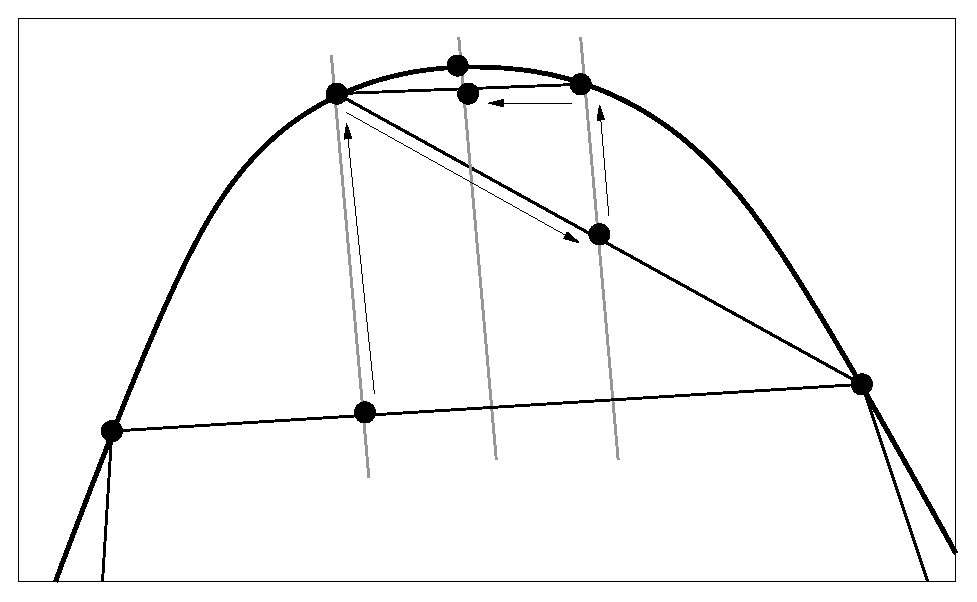
\includegraphics[width=0.6\textwidth]{figs/bisec1.eps}}
\caption{Combined subdivision and Newton method for locating special points of type 2.}
\label{frank:fig1}
\end{figure}


%%%%%%%%%%%%%%%%%%%%%%%%%%%%%%%%%%%%%%%%%%%%%%%%%%%%%%%%%%%%%%%%%%%%%%%
%%%%%%%%%%%%%%%%%%%%%%%%%%%%%%%%%%%%%%%%%%%%%%%%%%%%%%%%%%%%%%%%%%%%%%%






%%%%%%%%%%%%%%%%%%%%%%%%%%%%%%%%%%%%%%%%%%%%%%%%%%%%%%%%%%%%%%%%%%%%%%%
%%%%%%%%%%%%%%%%%%%%%%%%%%%%%%%%%%%%%%%%%%%%%%%%%%%%%%%%%%%%%%%%%%%%%%%

\newcommand{\mpbvp}{{\scshape Mpbvp}}

\section{Collocation core mpbvp}

\subsection{Discretisation of segmented BVPs}

Segmented ODE over $r$ segments:
%
\begin{eqnarray*}
\dot{x}_j & = & f_j(x_j,\lambda_j), \quad t\in[0,1], \quad j=1,\dots,r,
\end{eqnarray*}
%
$f:\R^n\times R^m\to\R^n$. Right-hand sides $f_j$ don't need to be pairwise different. 

\ToDo{different sets of parameters not supported yet [note made in todo list]}

Segmented ODE with variational equation:
%
\begin{eqnarray*}
\dot{x}_j & = & f_j(x,\lambda), \\
\dot{M}_j & = & \left(f_j\right)_x(x,\lambda), \\
M_j(0) + M_j(1) + \int_{0}^{1} M_j(\tau)^T M_j(\tau) \: d\tau
	& = & 3 I_{n\times n}, \quad t\in[0,1], \quad j=1,\dots,r,
\end{eqnarray*}
%
$f:\R^n\times R^m\to\R^n$, $M(t)\in\R^{n\times n}$.

Toolbox \mpbvp\ constructs a discretisation for segmented ODEs and their variational equation. Boundary conditions for the segmented orbits must be provided by toolboxes that utilise \mpbvp. The collocation system is constructed in class \class{coll}.

Discretised system over one segment (very compact functional notation):
%
\begin{eqnarray*}
T \cdot \kappa(t) \cdot f(W\disc{x},\lambda) - \dot{W}\disc{x} & = & 0, \\
T \cdot \kappa(t) \cdot f_x(W\disc{x},\lambda)\cdot W\disc{M} - \dot{W}\disc{M} & = & 0, \\
W\disc{M}(0) + W\disc{M}(1) + \left(\sum_{i} \omega(t_i) \cdot
	(W\disc{M})(t_i)^T (W\disc{M})(t_i)\right) - 3 I_{n\times n}
	& = & 0,
\end{eqnarray*}
%
where $W$ maps the supporting points in $\disc{x}$ to the values of $x(t)$ at the collocation points, $\dot{W}$ maps the supporting points to the values of the derivative $\dot{x}(t)$ at the collocation points, $T$ is the time of flight over one segment, $\kappa$ is a piecewise constant function, and $\omega(\tau)$ are the rescaled Gau\ss\ integration weights at collocation point $\tau$.

The use of $T$ and $\kappa$ introduces a double scaling as follows:
\begin{enumerate}
\item The scaling $$T\cdot \dots$$ maps the unit interval $\tau\in[0,1]$ onto the actual time interval $t\in[0,T]$.
\item The piecewise constant scaling $$\kappa(\tau)\cdot\dots$$ is an (inverse) blow-up scaling that maps the uniform reference mesh $$ \theta_k = 2k, \quad k=0,1,\dots,\mathrm{NTST}, $$ with equal-in-length subdivisions $\theta_k - \theta_{k-1} = 2$ onto a non-uniform mesh $$0 = \tau_0 < \tau_1 < \dots < \tau_{\mathrm{NTST}} = 1$$ of collocation intervals. Hence, the scaling function $\kappa$ satisfies $$ 2\cdot \mathrm{NTST}\cdot \int_0^1\kappa(\tau)\:d\tau = 1$$ and $\kappa(\tau)>0$ for all $\tau\in[0,1]$.

There are several reasons for the blow-up scaling in this way:
\begin{itemize}
\item The collocation interval over one interval can be shifted to $\theta\in[-1,1]$. Hence, the linear maps from the base points onto the collocation points and onto the derivative at the collocation points are matrices that do not change over the intervals.
\item For $\mathrm{NTST}\to\infty$ all derivatives of the collocation polynomials $p(\theta)=a_0+a_1 \theta + \dots + a_n\theta^n$ and, hence, all coefficients $a_k$, $k\geq 1$, will go to zero. This is not true for a collocation in $\tau$, where these coefficients will, in general, go to constants different from zero.
\item Adaptation will most likely be based on computing the coefficients $a_k$, $k\geq 1$. This computation involves divided differences at some point, which is stable for $\mathrm{NTST}\to\infty$ if the differences are of order ${\cal{O}}(1)$. We achieve this by keeping the length of the collocation interval fixed.
\end{itemize}
\end{enumerate}

BVPs can be set-up with or without variational equation. If variational equation is included, we have three different collocation systems, depending on their purpose:
%
\begin{enumerate}
\item For \emph{computing} an \emph{initial solution} $M(t)$ we perform a homotopy in $\beta : 0\to 1$ with the equation
%
\begin{eqnarray*}
\beta \cdot T_0 \cdot \kappa(t) \cdot f_x(W\disc{x}_0,\lambda)\cdot W\disc{M} - \dot{W}\disc{M} & = & 0, \\
W\disc{M}(0) + W\disc{M}(1) + \left(\sum_{i} \omega(t_i) \cdot
	(W\disc{M})(t_i)^T (W\disc{M})(t_i)\right) - 3 I_{n\times n}
	& = & 0,
\end{eqnarray*}
%
where $\disc{x}_0$ is an initial segmented solution to a BVP and we use the initial solution $M(t)|_{\beta=0} \equiv I_{n\times n}$ for the homotopy. This is coded in the set of functions starting with \class{var1}.

\item For \emph{tracking} $M$ for use in monitor functions of type \emph{regular} or \emph{singular} we use a \emph{decoupled} equation
%
\begin{eqnarray*}
T \cdot \kappa(t) \cdot f(W\disc{x},\lambda) - \dot{W}\disc{x} & = & 0, \\
T \cdot \kappa(t) \cdot f_x(W\disc{y},\mu)\cdot W\disc{M} - \dot{W}\disc{M} & = & 0, \\
W\disc{M}(0) + W\disc{M}(1) + \left(\sum_{i} \omega(t_i) \cdot
	(W\disc{M})(t_i)^T (W\disc{M})(t_i)\right) - 3 I_{n\times n}
	& = & 0,
\end{eqnarray*}
%
where we set $\disc{y}\from \disc{x}$ and $\mu\from \lambda$ in the second equation after each Newton step. This is done implicitly, we simply omit the the derivatives of the second equation with espect to~$\disc{x}$ and~$\lambda$, which leads to a decoupled system of linear equations. This is always well posed, because the variational equation always has a unique solution. Also, since we ignore derivatives with respect to parameters, the tangent vector $\xi$ is computed correctly. That is, the components of $M$ in $\xi$ are zero, which means that the computation of $M$ is \emph{slaved} to the computation of $x$ [We need to show this.]. This is coded in the set of functions starting with \class{var2}.

\item For \emph{using} $M$ in monitor functions and constraints we use the full collocation system as stated above, including all second-order derivatives in the linearisation. This is coded in the set of functions starting with \class{var}.
\end{enumerate}

The construction of a collocation system and its initial solution is split into individual steps as to allow switching between different modes of computing the variational equation in restarted computations.

\subsection{Multipliers of segmented periodic orbits}



%%%%%%%%%%%%%%%%%%%%%%%%%%%%%%%%%%%%%%%%%%%%%%%%%%%%%%%%%%%%%%%%%%%%%%%
%%%%%%%%%%%%%%%%%%%%%%%%%%%%%%%%%%%%%%%%%%%%%%%%%%%%%%%%%%%%%%%%%%%%%%%






%%%%%%%%%%%%%%%%%%%%%%%%%%%%%%%%%%%%%%%%%%%%%%%%%%%%%%%%%%%%%%%%%%%%%%%
%%%%%%%%%%%%%%%%%%%%%%%%%%%%%%%%%%%%%%%%%%%%%%%%%%%%%%%%%%%%%%%%%%%%%%%

\section{Acknowledgements}

FS was supported by EPSRC grant EP/D063906/1.

\section{Contact}

Frank Schilder, Department of Mathematics,
University of Surrey,
Guildford, Surrey \mbox{GU2 7XH},
United Kingdom \\
(f.schilder@surrey.ac.uk)

\vspace{2ex}\noindent Other author(s).

%%%%%%%%%%%%%%%%%%%%%%%%%%%%%%%%%%%%%%%%%%%%%%%%%%%%%%%%%%%%%%%%%%%%%%%%%%%%%%

\appendix
\renewcommand{\theequation}{\Alph{section}.\arabic{equation}}

%%%%%%%%%%%%%%%%%%%%%%%%%%%%%%%%%%%%%%%%%%%%%%%%%%%%%%%%%%%%%%%%%%%%%%%%%%%%%%

\bibliographystyle{abbrv} % plain alpha abbrv acm
\bibliography{references}

%%%%%%%%%%%%%%%%%%%%%%%%%%%%%%%%%%%%%%%%%%%%%%%%%%%%%%%%%%%%%%%%%%%%%%%%%%%%%%
\end{document} 

